\documentclass[a4paper, 11pt, ngerman, fleqn]{article}
\usepackage[utf8]{inputenc}
\usepackage{babel,ngerman}
\usepackage{ngerman}
\usepackage{coordsys,logsys,color}
\usepackage{hyperref}
\usepackage{texdraw}
\usepackage{fancyhdr}
\usepackage{graphicx}
\input{txdtools}

\NeedsTeXFormat{LaTeX2e}
\ProvidesPackage{hyperref}
\definecolor{darkblue}{rgb}{0,0,.6}
\hypersetup{pdftex=false, colorlinks=true, breaklinks=true, linkcolor=darkblue, menucolor=darkblue, urlcolor=darkblue, citecolor=darkblue}

\pagestyle{fancy}

%\renewcommand{\familydefault}{cmss}

\definecolor{fgcgray}{rgb}{0.4, 0.4, 0.4}
\definecolor{warning}{rgb}{0.9, 0.1, 0.0}
\definecolor{bgctitle}{rgb}{0.5, 0.5, 0.5}
\definecolor{fgctitle}{rgb}{0.95, 0.95, 0.95}
\newcommand{\titlefont}[1]{\textcolor{fgctitle}{\fontfamily{cmss}\fontseries{bx}\fontshape{n}\fontsize{20.48}{0pt} \selectfont #1}}
\newcommand{\inversetitlefont}[1]{\textcolor{bgctitle}{\fontfamily{cmss}\fontseries{bx}\fontshape{n}\fontsize{20.48}{0pt} \selectfont #1}}

\addtolength{\oddsidemargin}{-1.0cm}
\addtolength{\evensidemargin}{-1.0cm}
\addtolength{\headwidth}{2.0cm}
\addtolength{\textwidth}{2.0cm}

\setlength{\parindent}{0cm}

\renewcommand{\labelitemi}{$\circ$}
\renewcommand{\labelitemii}{$\diamond$}

\newcommand{\spaceline}[1][8pt]{\vskip #1}
\newcommand{\comment}[1]{\spaceline[5pt] \textcolor{fgcgray}{\scriptsize #1} \spaceline[15pt]}
\newcommand{\attrname}[1]{\textcolor{fgcgray}{\scriptsize #1}}


\makeatletter

\newcommand*{\project}[1]{\gdef\@project{#1}}
\newcommand*{\version}[1]{\gdef\@version{#1}}
\newcommand*{\home}[1]{\gdef\@home{#1}}
\newcommand*{\homeref}[1]{\gdef\@homeref{#1}}

\def\@maketitle{
  %\begin{titlepage}
  \begin{center}
    \colorbox{bgctitle}{
      \parbox{\textwidth}{
        \spaceline
        \centering{\titlefont{\@title}}
        \par
        \spaceline
      }
    }
    \colorbox{white}{
      \parbox{\textwidth}{
        \spaceline
        \centering{\inversetitlefont{\@project}}
        \par
        \spaceline
      }
    }
  \end{center}
  \spaceline[1.5em] {
    \begin{flushright}
    \begin{tabular}[t]{rl}
      \attrname{Projekt:} & \@project ~ \@version \\
      \attrname{Autor:} & \@author \\
      \attrname{letzte "Anderung:} & \@date
    \end{tabular}
    \end{flushright}
    \par
  }
  \spaceline[5.5em]
  %\end{titlepage}
}

\setcounter{secnumdepth}{4}
\setcounter{tocdepth}{4}

\newcounter{subsubsubsection}[subsubsection]
\def\subsubsubsectionmark#1{}
\def\thesubsubsubsection{\thesubsubsection .\arabic{subsubsubsection}}
\def\subsubsubsection{\@startsection{subsubsubsection}{4}{\z@}{-3.25ex plus -1 ex minus -.2ex}{1.5ex plus .2ex}{\normalsize\bf}}
\def\l@subsubsubsection{\@dottedtocline{4}{4.8em}{4.2em}}

\makeatother

\everytexdraw{
  \drawdim cm \linewd 0.01
  \arrowheadtype t:T
  \arrowheadsize l:0.2 w:0.2
  \setgray 0.5
}

\newcommand{\xheight}{0.6}
\newcommand{\xlength}{0.6}
\newcommand{\yheighta}{1.0}
\newcommand{\yheightb}{0.8}
\newcommand{\yheightc}{0.6}
\newcommand{\yheightd}{0.5}
\newcommand{\yheighte}{0.4}
\newcommand{\yheightf}{0.35}

\newcommand{\xhline}{\rlvec({\xlength} 0)}
\newcommand{\xharrow}{\ravec(0.7 0)}
\newcommand{\xnext}{%\rlvec(0.05 0) \lpatt(0.04 0.04) \rlvec(0.15 0) \lpatt()
}

\newcommand{\xtext}[3][\xheight]{
  \bsegment
    \bsegment
      \setsegscale 0.5
      \textref h:L v:C  \htext({\xheight} -0.1){#3}
    \esegment
    \setsegscale 0.5 \lvec(0 #1)
    \setsegscale 1
    \rlvec(#2 0) \rlvec(0 -#1) \rlvec(-#2 0) \lvec(0 0)
    \savepos(#2 0)(*@x *@y)
  \esegment
  \move(*@x *@y)
}

\newcommand{\bxtext}[3][\xheight]{
  \setgray{0.1}
  \linewd{0.026}
  \xtext[\xheight]{#2}{#3}
  \linewd{0.01}
  \setgray{0.5}
}

\newcommand{\xstartpage}{\bxtext{2.1}{Startseite}}
\newcommand{\xmainpage}{\bxtext{2.3}{Hauptseite}}
\newcommand{\xusermenu}{\bxtext{2.9}{Benutzermenu}}
\newcommand{\xgamelist}{\bxtext{2.2}{Spieleliste}}
\newcommand{\xportfolio}{\bxtext{2.0}{Portfolio}}
\newcommand{\xaccount}{\xtext{3.8}{Kennung per \textsl{eMail}}}


\begin{document}
  \lhead{\sc{Virtual Reality für Sensordatenanalyse}}
%\cfoot{-~\thepage~-}
\title{Pflichtenheft}
\project{Virtual Reality für Sensordatenanalyse}
\version{0.1}
\author{Alexej Gluschkow, Fabian Klopfer, Gero Birkhölzer, Lisa-Maria Mayer}
\maketitle
%\thispagestyle{empty}
%~
%\newpage
%\tableofcontents
 \newpage
  \textcolor{warning}{Es muss zu jeder weiteren Produktfunktion ein konkreter Testfall hinzugefügt werden ...}
  \tableofcontents \newpage
  \section{Objective}

\comment{Vom Blatt}

\textbf{}

\subsection{Mandatory Criterias}

\begin{itemize}
  \item Comm sensor/app
  \item Sensordaten visualisierung (mehr als eine)
  \item Exploration (mit Joystick)
  \item Comm app/webVR/sensor(als Beacon)
  \item Positionapproximation durch beacons

  \item VR-Mode
  \begin{itemize}
    \item The VR-World shall model at least two different rooms and a connect hallway.
    \item The VR-World shall be viewed inside a web browser and from the App.
    \item The VR-World shall have a stereoscopic 3D-Mode of the World.
    \item While viewing the VR-World the user shall be able to look around using the gyro senor of his phone to pan the camera around.
    \item While the App is not in stereoscopic 3D mode the User shall be able to click and drag to pan the camera around.
    \item The User shall be able to move the camera inside the Vr-World by using his controller.
    \item The Data fechted from the Sensor shall be displayed inside the VR-World.
    \item There shall be at least two different representations the data from the Sensor.
    \item The VR-World shall represent at least two different real world rooms.
    \item The User shall be able to easily switch between stereoscopic 3D and normal 3D mode.
    \item The App shall be in fullscreen mode, while in VR-Mode.
    \item While in stereoscopic 3D-Mode the user shall be able to exit it by looking for 5 seconds at the cross under his feet.
  \end{itemize}
  \item Other
  \begin{itemize}
    \item The App shall not dimm the screen while inside VR-Mode.
    \item
  \end{itemize}
\end{itemize}

\subsection{Desired Criterias}

\begin{itemize}
  \item The VR-World represents a whole corridor with more then two rooms.
  \item AR
  \item TI sensor als bewegung
\end{itemize}

\subsection{Boundary Criterias}

\begin{itemize}
  \item Keine persistente Speicherung
\end{itemize}
 \newpage
  \section{Produkteinsatz}

\comment{Welche Anwendungsbereiche (Zweck), Zielgruppen (Wer mit welchen Qualifikationen), Betriebsbedingungen (Betriebszeit, Aufsicht)?}

\comment{Beacons}

\subsection{Anwendungsbereiche}


\subsection{Zielgruppen}

\subsection{Betriebsbedingungen}

\begin{itemize}
  \item
\end{itemize}
 \newpage
  \section{Product enviroment}

\comment{Welche Software, Hardware und Orgware wird benötigt?}
\comment{Blatt}

\subsection{Software}

The App will be developed for Android.

  \begin{itemize}
    \item Android 4.4 or higher
    
    \item \textbf{} \textit{(mind. Version 4.0.5)}
  \end{itemize}

\subsection{Hardware}

  \begin{itemize}
    \item Smartphone with Bluetooth
    \item (Some device to view the VR-part properly)
    \item
  \end{itemize}

\subsection{Orgware}

\begin{itemize}
  \item
\end{itemize}
 \newpage
  \section{Produktfunktionen}

\comment{Was leistet das Produkt aus Benutzersicht?}
\comment{Beacon und blatt}
\subsection{Settings}

The User can set the following Options:
\begin{description}
  \item[/F0100/] 
	\textit{Sensor:} The User can set, which data should be displayed in the VR-World (Temperature, etc.)
\end{description}

\subsection{VR-World}

\begin{description}
  \item[/F0300/]
    \textit{Look around:} The User can look around in the VR-World by touching and draging on the Screen or by moving his head around, while he is in VR mode.
\end{description}

\begin{description}
  \item[/F0310/]
    \textit{Move inside VR-World:} The User can move inside the VR-World by tilting the joystick of his controller forward. Turning will be done by looking around with the VR-headset.
\end{description}

\begin{description}
  \item[/F0320/]
    \textit{Switch Data representation:} The User can switch between two different respresentations of the bluetooth data from the sensor by pressing the A-Button on his controller.
\end{description}

\begin{description}
  \item[/F0330/]
    \textit{Exit VR view:} The User can exit the VR view by pressing the x in the top right corner of the screen or by looking for 5 seconds directly on the x under his feet.
\end{description}

\begin{description}
  \item[/F0340/]
    \textit{Enter stereoscopic VR view:} The User can switch from fullscreen VR view to stereoscopic by pressing the button in the lower right corner or by pressing the A-Button on his controller.
\end{description}

\begin{description}
  \item[/F0350/]
    \textit{Exit stereoscopic VR view:} The User can leave stereoscopic VR view by pressing the back button on his device or by touching the back button in the top left corner.
\end{description}
 \newpage
  \section{Produktdaten}

\comment{Was speichert das Produkt (langfristig) aus Benutzersicht?}
\comment{noch nichts; evtl 4. einbinden}

Jeder Punkt \textbf{/D???/} stellt im Prinzip einen Datensatz dar.

\begin{description}
  \item[/D010/]
    \textit{Benutzerdaten:} Alle Informationen zu einem Benutzer:
    \begin{itemize}
      \item \textbf{BenutzerID} \textit{(eindeutig)}
      \item Kennung
        \begin{itemize}
          \item \textbf{Benutzername} \textit{(eindeutig)}
          \item \textbf{Passwort} \textit{(verschlüsselt)}
        \end{itemize}
    \end{itemize}
\end{description}
 \newpage
  \section{Produktleistungen}

\comment{Welche zeit- und umfangsbezogenen Anforderungen gibt es?}
\comment{Milestones, Leistung auf realer HW, bsp: mehr als 5 FPS}
\begin{description}
  \item[/L100/] The VR-View should run with at least 30 FPS.
\end{description}

\begin{description}
  \item[/L100/] The VR-World should be expandable so that new Rooms can be added.
\end{description}


 \newpage
  \section{User interface}

\subsection{Structure}

A small overview of the menu Structure.

\subsubsection{Start screen}

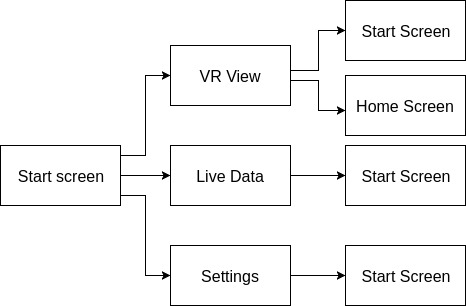
\includegraphics[scale=0.5]{pics/startscreen.jpg}

\subsubsection{VR-Mode}

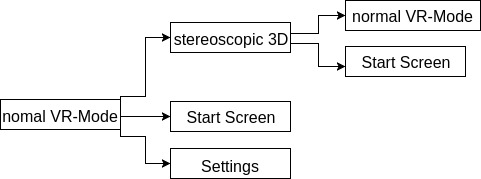
\includegraphics[scale=0.5]{pics/Vr-Mode.jpg}


\subsubsection{Live Data}

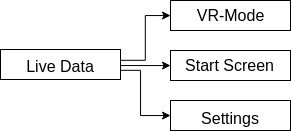
\includegraphics[scale=0.5]{pics/Live_Data.jpg}

\subsubsection{Settings}

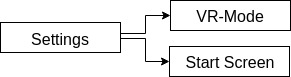
\includegraphics[scale=0.5]{pics/Settings.jpg}

\newpage
\subsection{Layout}

A mockup of the Start up screen.
\\
\\
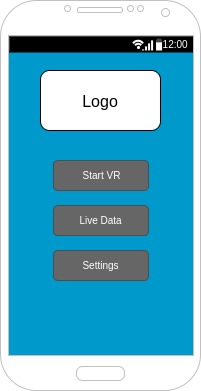
\includegraphics[scale=0.5]{pics/startScreen_mockup.jpg}
\\

And a mockup of the stereoscopic Vr-Mode.
\\
\\
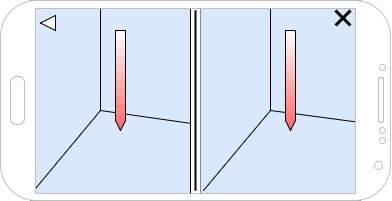
\includegraphics[scale=0.5]{pics/VRView_mockup.jpg}
 \newpage
  \section{Qualitätszielbestimmungen}

\comment{Auf welche Qualitätsanforderungen (Zuverlässigkeit, Robustheit, Benutzungsfreundlichkeit, Effizienz, ...) wird besonderen Wert gelegt?}

\begin{center}
 \begin{tabular}{l|c|c|c|c}
  ~ & sehr wichtig & wichtig & weniger wichtig & unwichtig\\
  \hline \hline
  \textit{Robustheit}~ & \textbf{X}~ &  ~ ~ ~ &  ~ ~ ~ &  ~ ~ ~ \\
  \hline
  \textit{Zuverlässigkeit}~ & \textbf{X}~ &  ~ ~ ~ &  ~ ~ ~ &  ~ ~ ~ \\
  \hline
  \textit{Korrektheit}~ & \textbf{X}~ &  ~ ~ ~ &  ~ ~ ~ &  ~ ~ ~ \\
  \hline
  \textit{Benutzungsfreundlichkeit}~ &  ~ ~ ~ & \textbf{X}~ &  ~ ~ ~ &  ~ ~ ~ \\
  \hline
  \textit{Effizienz}~ &  ~ ~ ~ & \textbf{X}~ &  ~ ~ ~ &  ~ ~ ~ \\
  \hline
  \textit{Portierbarkeit}~ &  ~ ~ ~ &  ~ ~ ~ & \textbf{X}~ &  ~ ~ ~ \\
  \hline
  \textit{Kompatibilität}~ &  ~ ~ ~ &  ~ ~ ~ & \textbf{X}~ &  ~ ~ ~ \\
 \end{tabular}
\end{center}
 \newpage
  \section{Globale Testszenarien und Testfälle}

\comment{Was sind typische Szenarien, die das Produkt erfüllen muss?}

Jede Produktfunktion \textit{/F????/} wird anhand von konkreten Testfällen \textit{/T????/} getestet.\\
Die dabei verwendeten Namen werden rein zufällig gewählt.

\begin{description}
  \item[/T????/]
    ...
\end{description}

\textcolor{warning}{Es muss zu jeder weiteren Produktfunktion ein konkreter Testfall hinzugefügt werden ...}
 \newpage
  \section{Entwicklungsumgebung}

\comment{Welche Software, Hardware und Orgware wird zur Entwicklung benötigt?}

Es wird darauf geachtet, dass alle Entwicklungstools quelloffen \textit{(Open Source)} sind.

\subsection{Software}

\begin{itemize}
  \item Plattform
    \begin{itemize}
      \item Java X.X
    \end{itemize}
  \item Tools
    \begin{itemize}
      \item \LaTeX
    \end{itemize}
  \item ...
    \begin{itemize}
      \item I
    \end{itemize}
\end{itemize}

\subsection{Hardware}

\begin{itemize}
  \item
\end{itemize}

\subsection{Orgware}

\begin{itemize}
  \item Terminliste
\end{itemize}
 \newpage
  \section{Quellen}

\comment{Spezielle, noch nicht abgedeckte Anforderungen.}

\begin{description}
	\item[Pflichtenheft Template]
	Simon K. Baur
	\href{http://www.linux-magazin.de/Media/Linux-Magazin/Files/latex}{Link}
\end{description}
 \newpage
  \section{Glossar}

\comment{Definition aller wichtigen Begriffe zur Sicherstellung einer einheitlichen Terminologie.}

\begin{description}
  \item[Fernspiele]
    
\end{description}

\end{document}
